\chapter{Flutter}
Firstly, this chapter contextualizes Flutter's unique approach within mobile development (Section~\ref{section::other_architectures}). 
Secondly, it presents an architectural overview of the framework (Section \ref{section::flutter_architecture}). 
Both explorations provide the reader with the necessary background knowledge in order to understand implementation choices of the clone application (detailed in Chapter \ref{chapter::implementation}) 
as well as particular eloborations in the study results (Chapter \ref{chapter::results}).

\section{Mobile Development Approaches} \label{section::other_architectures}
The following subsections depict the individual mobile development approaches (derived from \cite{Heitkoetter2013} and \cite{Cunha2018}).
Each technique can be placed along a spectrum of being built with web technologies on one and native technologies on the other end (see Figure \ref{fig::mobile_development_approach_spectrum}).\\
Generally, a higher reliance on native over web technologies corresponds to improved performance and usability as shown by \textcite{Heitkoetter2013}.

\begin{figure}
    \centering
    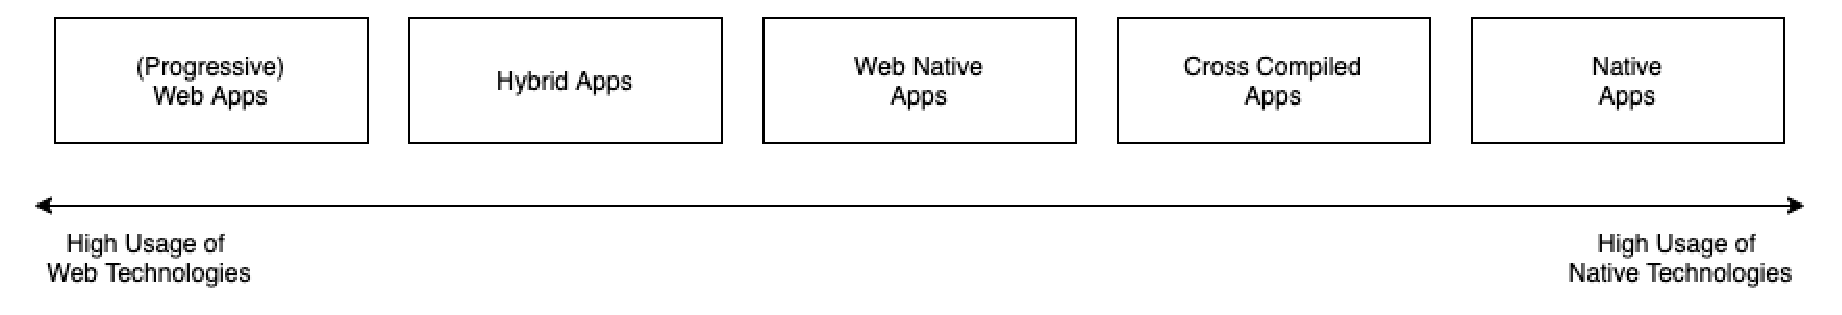
\includegraphics[width=\linewidth]{images/architectures/mobile_development_approaches.eps}
    \caption{Mobile Development Approach Spectrum}
    \label{fig::mobile_development_approach_spectrum}
\end{figure}


\subsection{Web App and Progressive Web App Approach} \label{subsection::web_apps}
Web apps are run and rendered in the browser. The underlying technologies are HTML, CSS and JavaScript with popular frameworks 
used for the development process such as Angualar (\cite{Angular2021}), React.js (\cite{React2021}) and Vue.js (\cite{Vue2021}). 
Relying on the Browser and an internet connection, they do not have access to hardware capabilites or the file system.\\
Progressive Web Apps (PWAs) function similarly to web apps but provide additional capabilities such as offline use, locally cached data, 
and push notifications. However, the feature set of PWAs is limited to the functionality exposed through the underlying browser.

\subsection{Hybrid Approach}
Hybrid Apps utilize the same technologies as web apps (see Subsection \ref{subsection::web_apps}), but they are rendered in a platform web view (see Figure \ref{fig:hybrid_architecture}). Additionally they provide the ability to 
interact with native APIs such as GPS and sensor data through a platform bridge (see Figure \ref{fig:hybrid_architecture}).
Unlike web apps, hybrid apps are shippable through official stores.
Popular framework choices for building Hybrid Apps include Ionic (\cite{Ionic2021}) and Cordova (\cite{Cordova2020}).

\begin{figure}
    \centering
    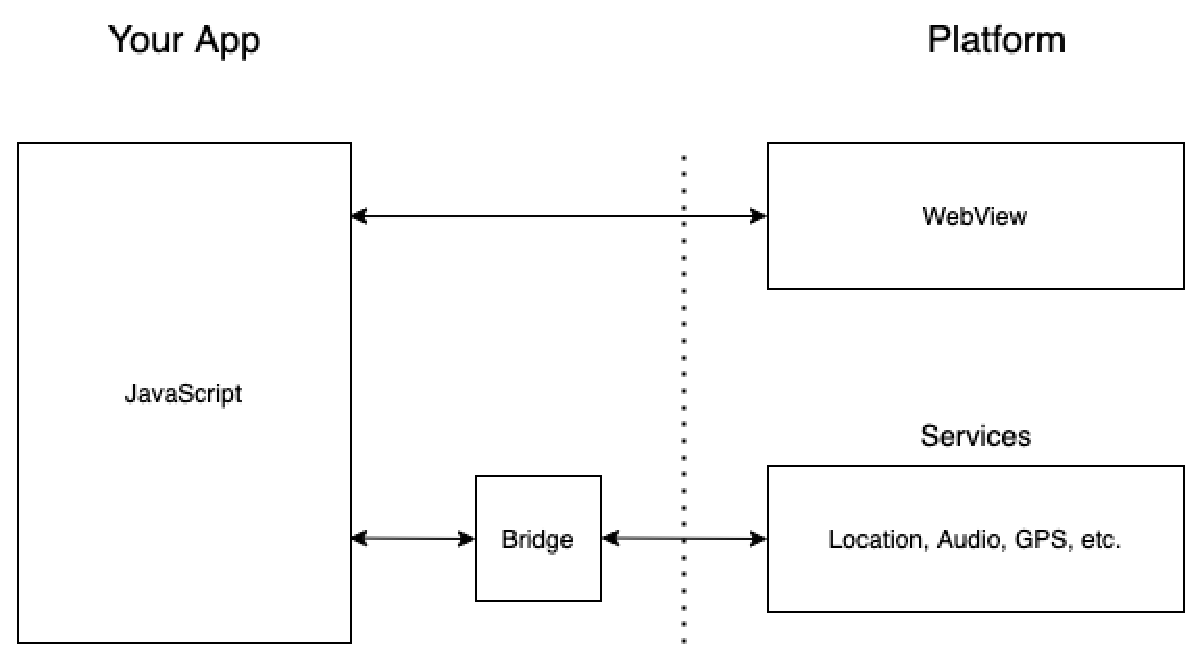
\includegraphics[width=.8\linewidth]{images/architectures/hybrid_architecture.eps}
    \caption{Mobile Hybrid Framework Architecture (adapted from \cite{Cunha2018}).}
    \label{fig:hybrid_architecture}
\end{figure}

\subsection{Web Native Approach} \label{subsection::web_native_apps}
Web Native Apps utilize the OEM components instead of web views for UI rendering while primarily using JavaScript.
This is achieved by using a platform bridge for the transpilation of JavaScript into native platform code allowing for OS level user interface component employment
and system services calls. 
Favored frameworks for building web native apps include React Native (\cite{ReactNative2021}) and Native Script (\cite{NativeScript2021}).

\begin{figure}
    \centering
    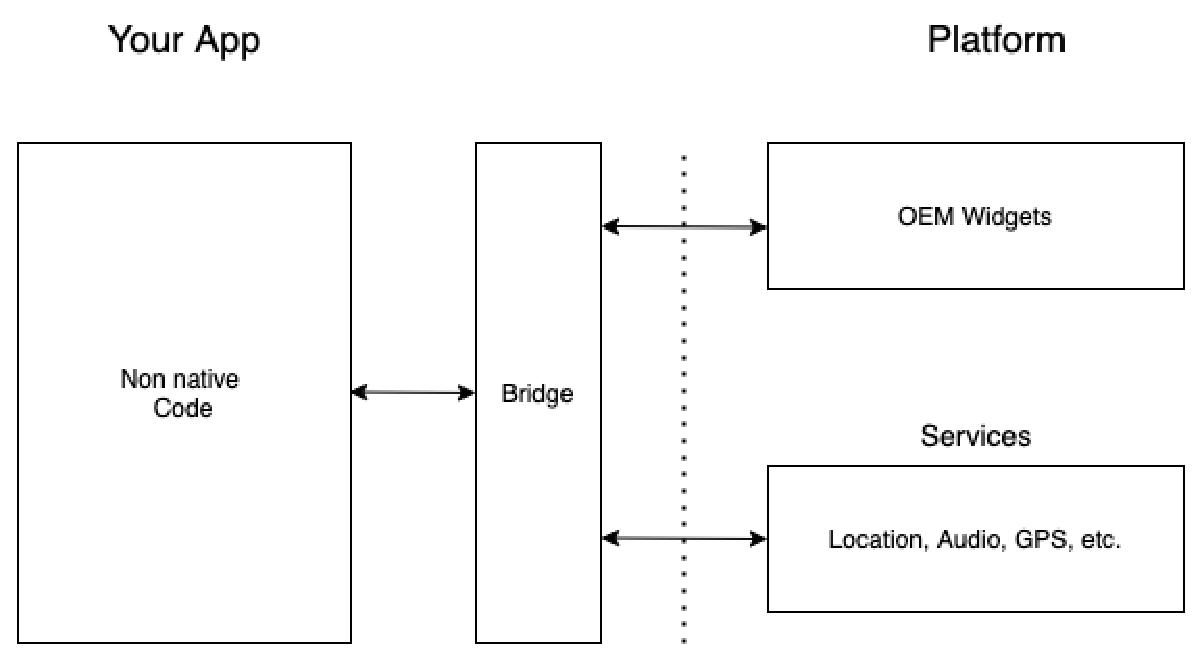
\includegraphics[width=.8\linewidth]{images/architectures/native_web_app_architecture.eps}
    \caption{Web Native and Cross Compiled Mobile Framework Architecture (adapted from \cite{Cunha2018}).}
    \label{fig:web_native_architecture}
\end{figure}

\subsection{Cross Compiled Approach} \label{subsection::cross_compiled_approach}
Generally, cross compiled apps take advantage of UI components and services from the underlying host platform similar to web native apps (see Subsection \ref{subsection::web_native_apps} and Figure \ref{fig:web_native_architecture}).
The OS plugin mechanism works by executing generated byte or machine code on the target device from a compiled language such as C\# (used for Xamarin, \cite{Xamarin2021}).\\
Flutter may be classified as a cross compilation based approach. However, it uniquely leaves the UI rendering process to its \textbf{Skia} graphics engine.
The framework's architecture and technicalities are further explained in Section \ref{section::flutter_architecture}.

\begin{figure}
    \centering
    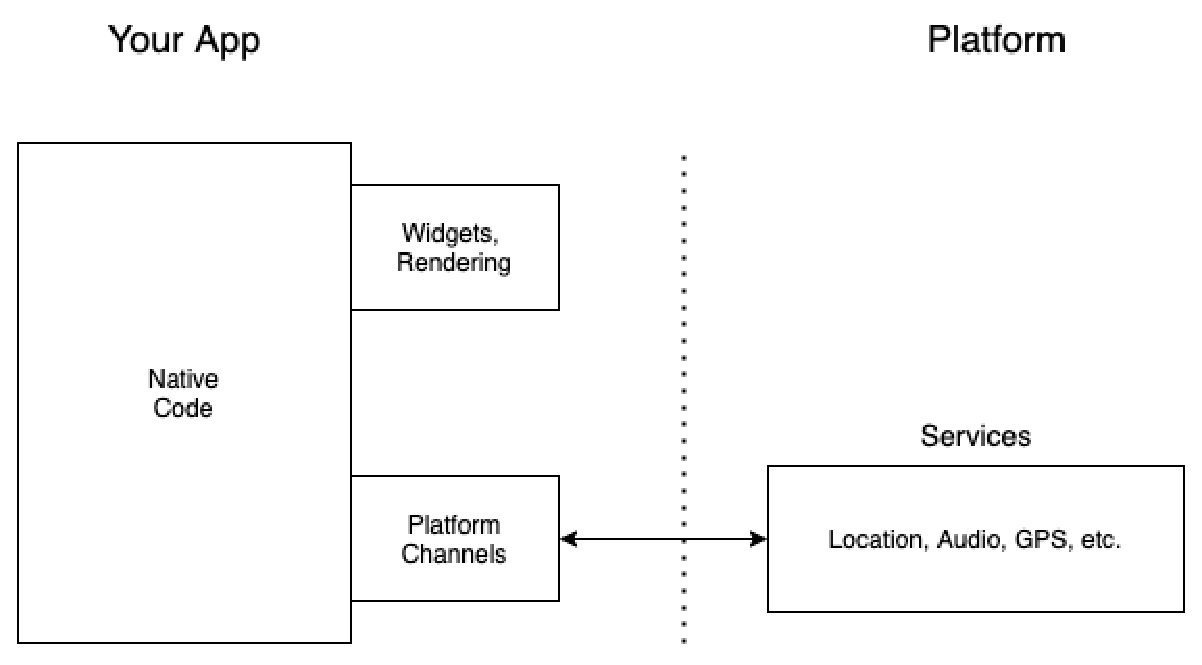
\includegraphics[width=.8\linewidth]{images/architectures/flutter_architecture.eps}
    \caption{Flutter Architecture (adapted from \cite{Cunha2018}).}
    \label{fig:flutter_architecture}
\end{figure}

\subsection{Native Approach}
The native approach is facilitated by the platform vendor and characterized by optimal OS integration through high hardware and software cohesion.
Separate technology stacks as well as programming languages are used for implementing apps natively. 
iOS supports Swift and Objective-C whereas Android supports Kotlin, Java and C++.



\begin{figure}
    \centering
    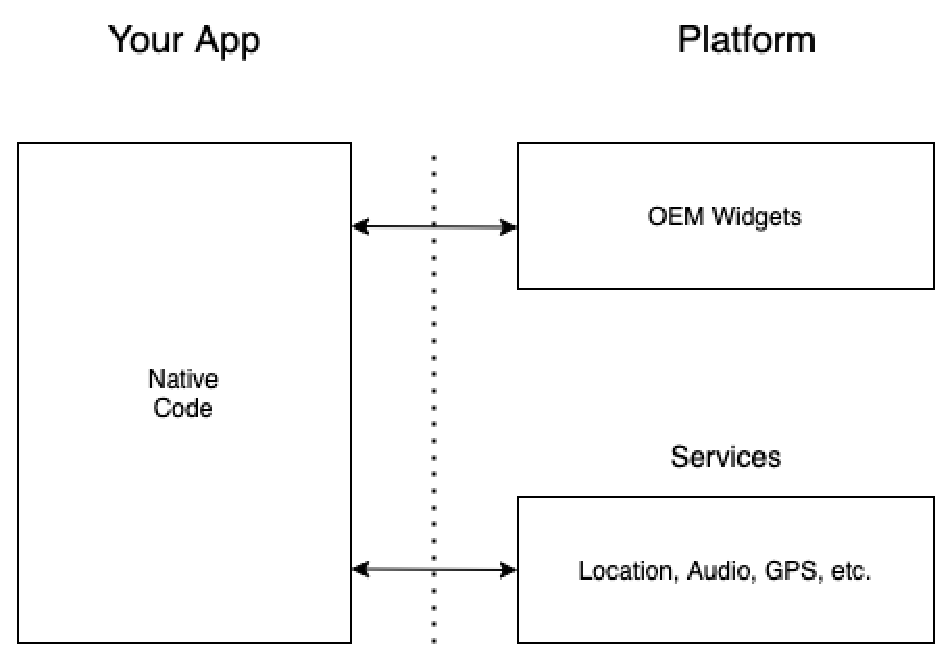
\includegraphics[width=.7\linewidth]{images/architectures/native_architecture.eps}
    \caption{Native Mobile Architecture (adapted from \cite{Cunha2018})}
    \label{fig:native_architecture}
\end{figure}

\section{Flutter Framework Architecture} \label{section::flutter_architecture}
Flutter's architecture is composed of three distinct layers: \textbf{framework}, \textbf{engine} and \textbf{embedder}. 
The framework is the top most layer which app developers interact with. It features animation and gesture APIs as well as structural and preconfigured platform specific UI components delivered through
the \textbf{Material} (Android) and \textbf{Cupertino} (iOS) package.\\
Below the framework layer lies the engine which is written in C and C++ allowing for the production of native binaries. 
This act of cross-compilation is Flutter's technical value proposition to increase execution performance as stated in 
Subsection \ref{subsection::cross_compiled_approach}. The engine layer includes \textbf{Skia} - a 2D graphics rendering engine which is also used by the Chrome, Mozilla Firefox and Android (\cite{Skia2021}).
Furthermore, Dart runtime management, system event interaction as well as platform channel services (described in \ref{subsection::method_channels}) are part of the engine layer.\\
The Embedder is the lowest layer of Flutter's architecture. Its sole purpose is to integrate the Flutter application into the platform-specific environment
by providing native plugins, thread setup and event loop interoperation.
Additionally, app package formatting is provided in the same way as for native apps. 
The host operating is thus not able to differentiate between a Flutter and a natively written app.

\begin{figure}
    \centering
    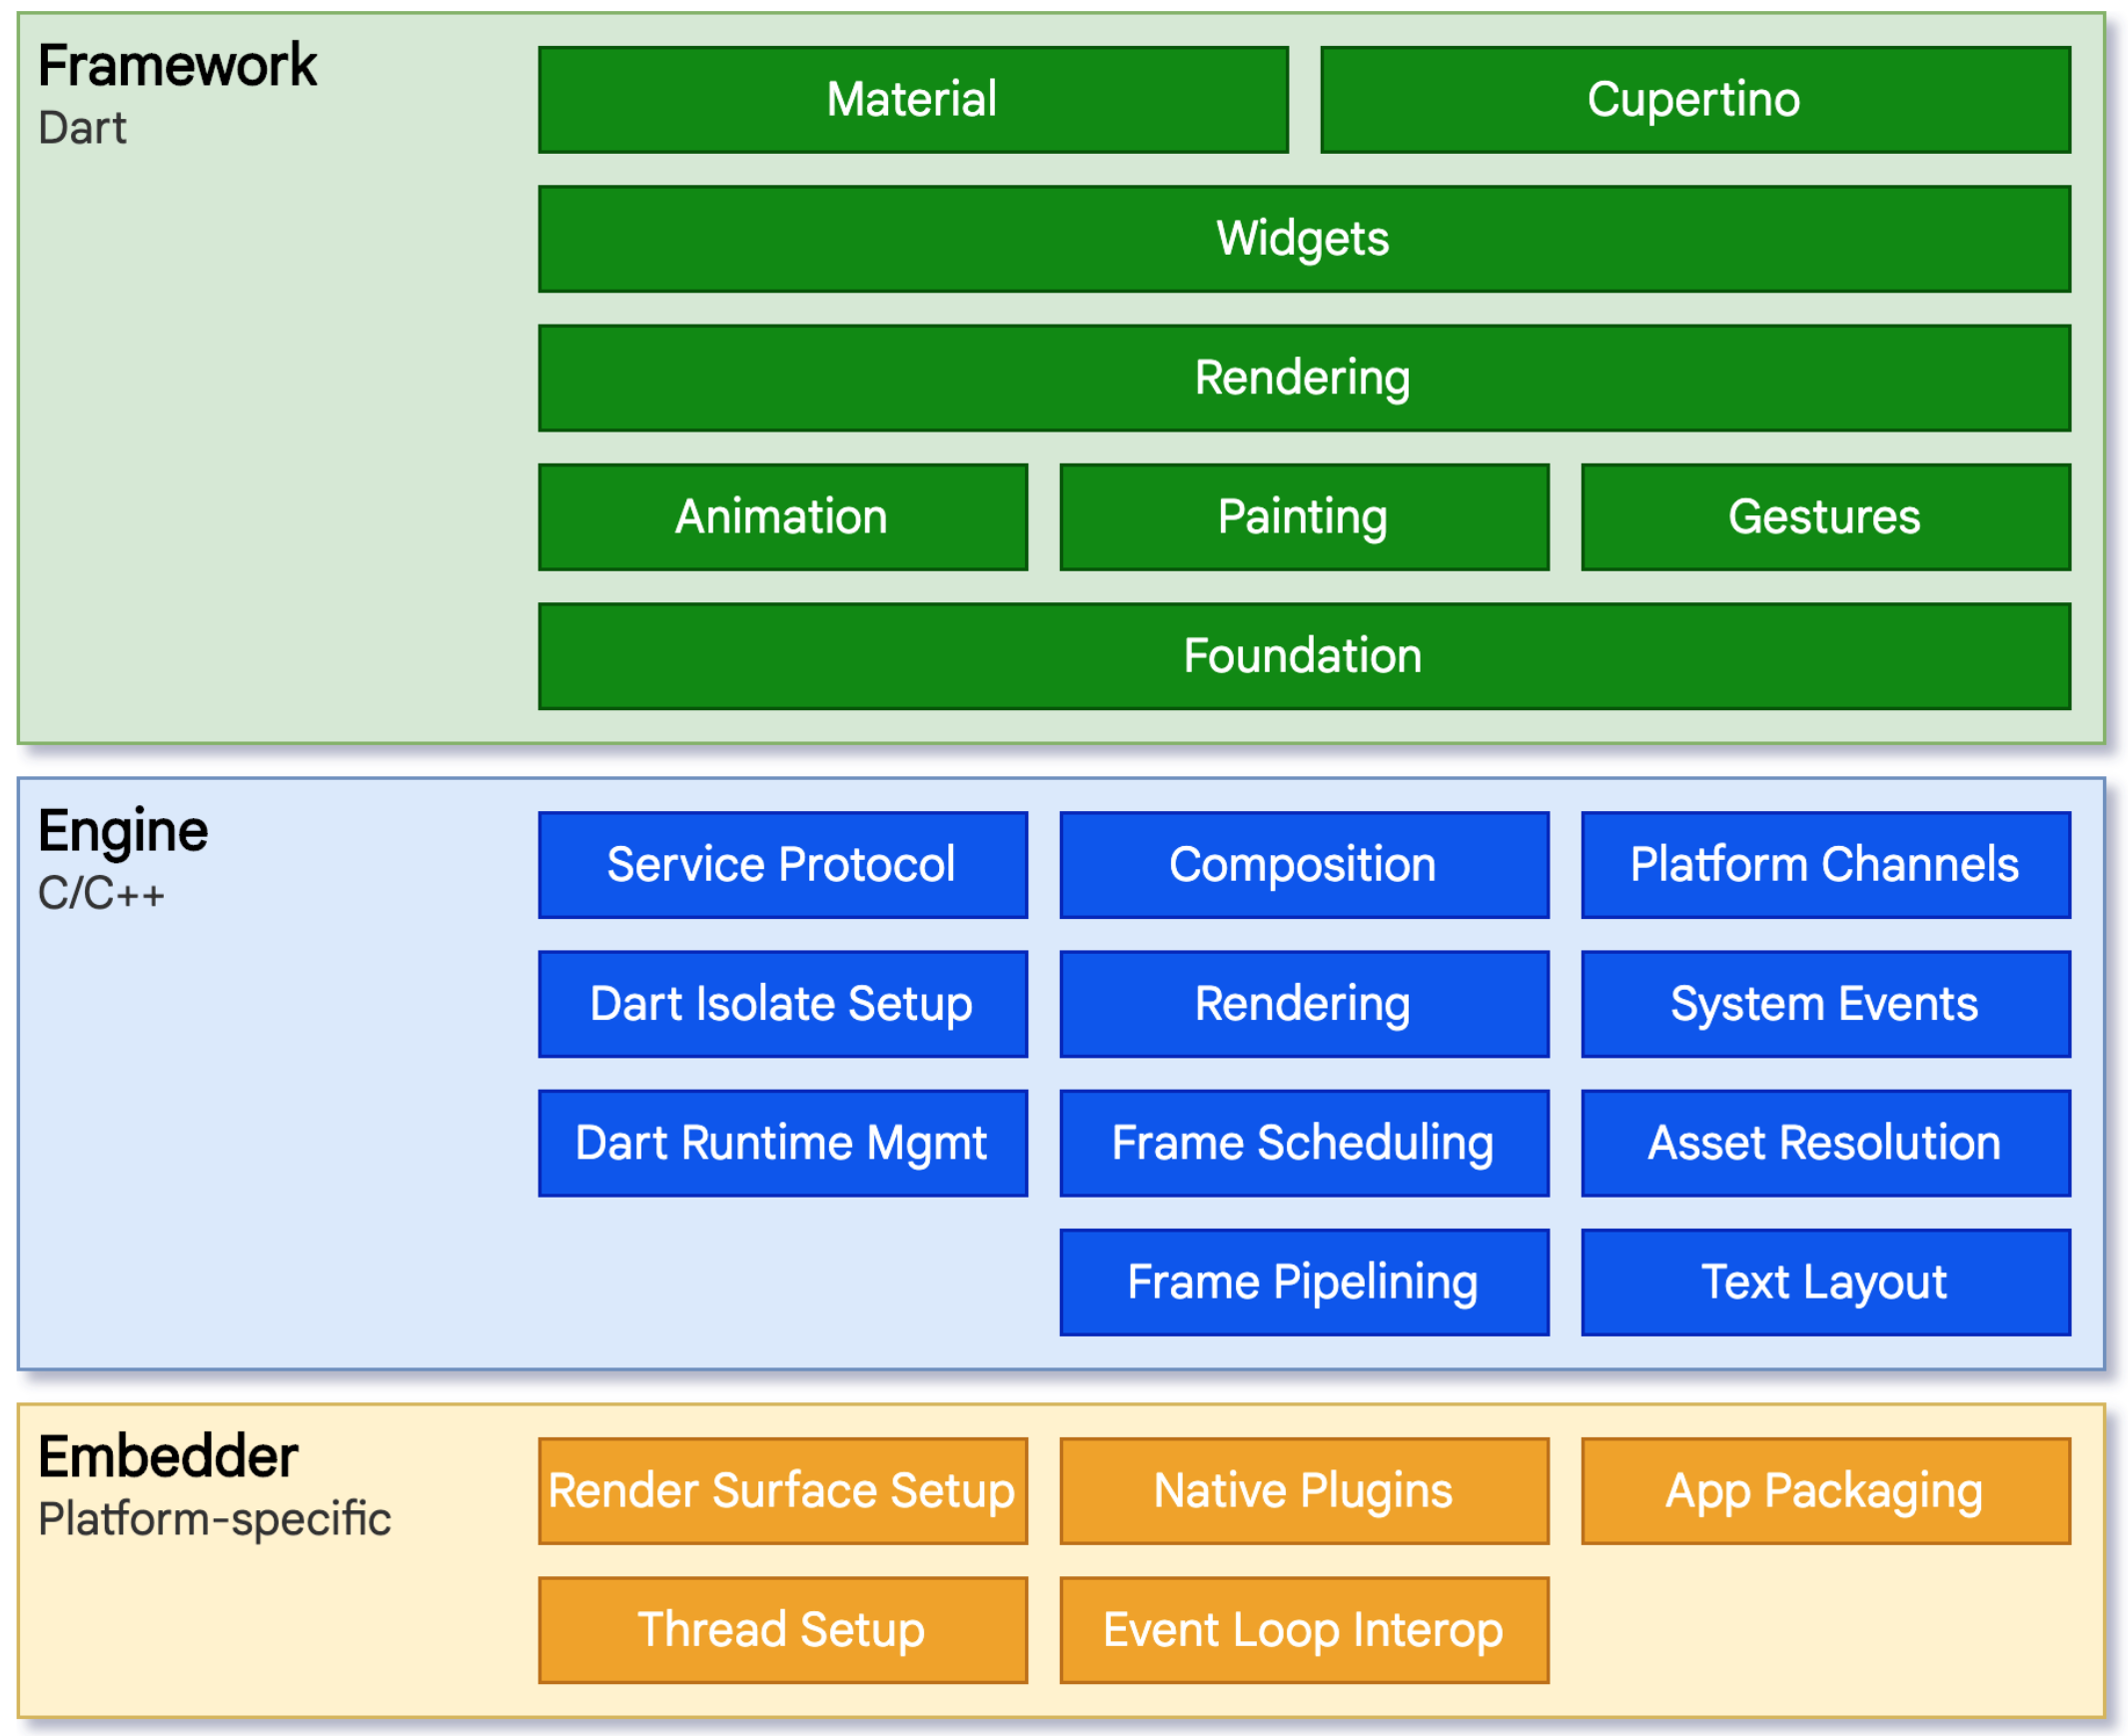
\includegraphics[width=\linewidth]{images/flutter_layered_architecture.eps}
    \caption{Flutter's Layered Architecture (adapted from \cite{FlutterArchitecture2021})}
    \label{fig:flutter_layered_architecture}
\end{figure}


\subsection{Programming Language and Compilation}
Flutter apps are written in Dart - a compiled multiparadigm programming language syntactically similar to Java (see \cite{DartLanguage2021}).\\
During Flutter development, apps run in the Dart Virtual Machine using Just-In-Time (JIT) compilation (\cite{DartLanguage2021}). 
This offers stateful \textbf{hot reload} which allows reloading the UI after code changes without needing to fully recompile the app leading to faster development cycles.\\
For release purposes, Flutter applications are Ahead-of-Time (AOT) compiled into native machine code including the Intel x86 and ARM CPU instruction sets in order to optimize production performance
(see \cite{FlutterArchitecture2021}).


\subsection{Rendering and UI State} \label{subsection::rendering_ui_state}
Flutter apps are fundamentally composed of widgets which declare structural, stylistic and layout elements for building the user interface. 
Each widget may have 0, 1 or multiple children which in turn create a tree structure of parent-child relationships. \\
For example, the information presented for each posting on the overview of the Kickdown app (see Figure \ref{fig:kickdown_overview_info_ui}) is built using a simple widget tree structure (see structural Diagram in Figure \ref{fig:kickdown_overview_info_ui_tree} and Code Snippet \ref{lst:code_snippet}):\\
A \textbf{Column} widget has the purpose of laying out 2 \textbf{Row} children vertically. Correspondingly, the Row widgets layout out their children horizontally. 
The first Row contains 2 \textbf{Text} widgets which represent the posting's title and current price of the car. 
Text widgets are terminal nodes as they have no further children\footnote{Technically both Text and Image do have an implicit single child widget which is created by the framework.}.
The second Row, contains another Text widget representing the location and a \textbf{CountdownLabel} which is a custom built widget abstracting away its internal complexity at its point of use.\\
The entry point of every Flutter app is either a \textbf{MaterialApp} or \textbf{CupertinoApp} widget which also marks the root of the tree.
Based on this tree structure Flutter can determine where and how elements should be drawn on screen, and instruct its graphics engine accordingly.
This concept alone is not yet sufficient to enable modern mobile applications with complex UI changes or animations 
based on asynchronous events like user interaction. 
Widgets are mappings from state to a UI representation using the abstraction of \textbf{RenderObjects}. When the state changes during runtime Flutter creates a new RenderObject tree, 
diffs it against the old one, and then redraws only its changes to the screen.
This reactive approach simplifies UI development in the sense that the developer does not need to keep track of UI state which can grow exponentially
with the increase of UI components on screen. 

\begin{figure}
    \centering
    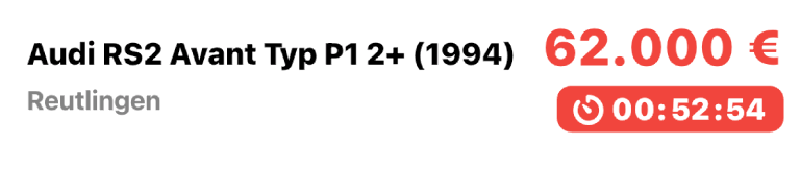
\includegraphics[width=.5\linewidth]{images/posting_information_UI.eps}
    \caption{Kickdown Posting Overview Car Information UI}
    \label{fig:kickdown_overview_info_ui}
\end{figure}

\begin{figure}[htbp]
    \begin{tabular}{p{0.5\textwidth}p{0.5\textwidth}}
        \begin{minipage}{.5\textwidth}
        \centering
        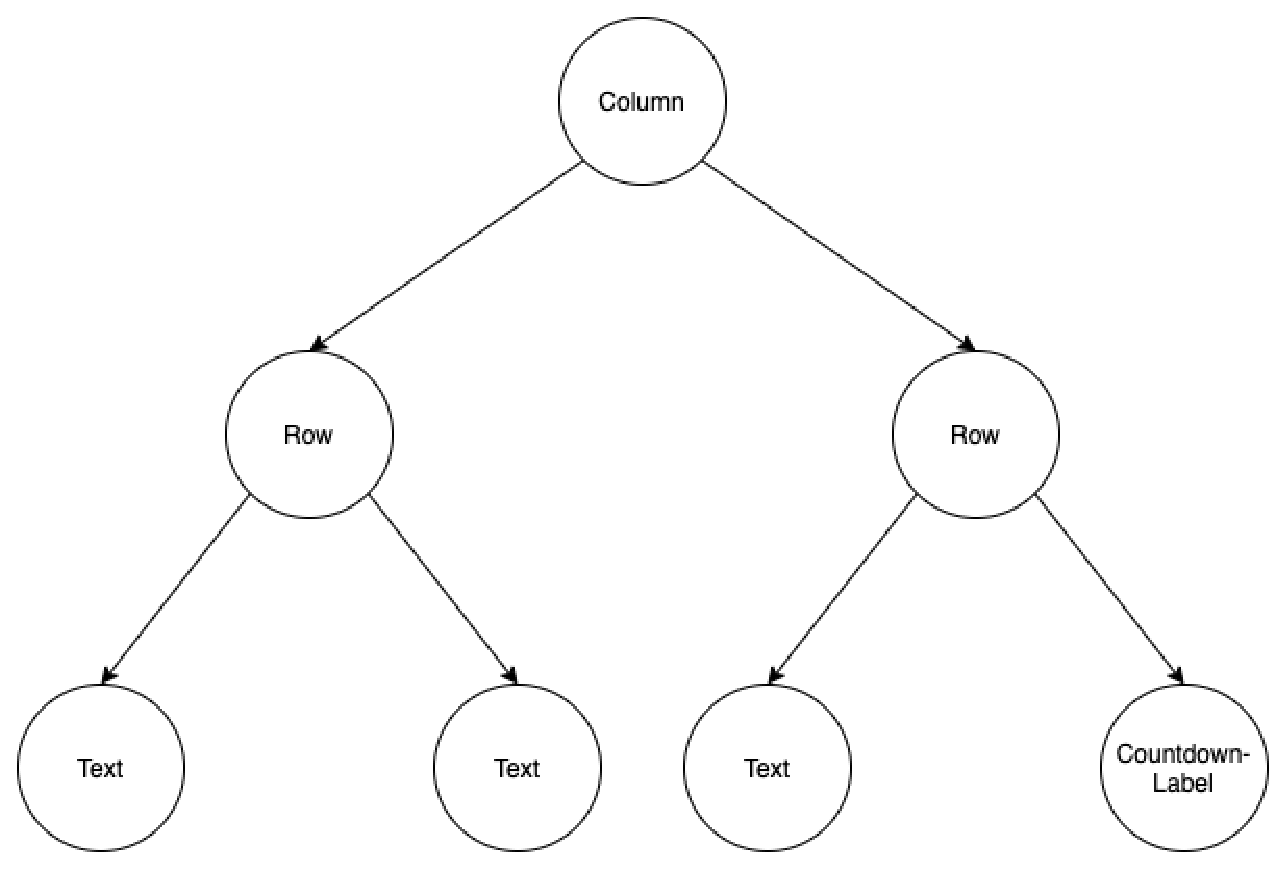
\includegraphics[width=\linewidth]{images/Kickdown_overview_info_ui_tree.eps}
        \caption{Widget Tree Structure Visualization of Code Snippet \ref{lst:code_snippet}}
        \label{fig:kickdown_overview_info_ui_tree}
        \end{minipage}
        &
        \begin{minipage}{.5\textwidth}
            \begin{lstlisting}[caption={Simplified Flutter Code for UI Layout shown in Fig. \ref{fig:kickdown_overview_info_ui}}\label{lst:code_snippet}]
            Column(
                children: [
                    Row(
                        children: [
                            Text("Audi RS2..."),
                            Text("62.000 €"),
                        ],
                    ),
                    Row(
                        children: [
                            Text("Reutlingen"),
                            CountdownLabel(...),
                        ]
                    )
                ],
            ),
            \end{lstlisting}
    \end{minipage}
    \end{tabular}
    \end{figure}

\subsection{Platform Specific Method Channels} \label{subsection::method_channels}
To utilize platform-specific APIs such as camera access, geolocation or other sensor data, Flutter communicates with the platform's native APIs via 
a method channel (see Figure \ref{fig:flutter_architecture}). 
This internal channel is used to execute code written in a host specific language. Thereby, Dart may be used to call Swift or Objective-C on iOS, and Kotlin or Java on Android (see \cite{PlatformChannel2021}).
Common functionalities are already provided by Flutter or third party packages (\cite{PubDev2021}). Additionally, custom platform integrations may be 
implemented as required.

\subsection{Flutter's Architectural Limitations}
As explained in Subsection \ref{subsection::rendering_ui_state}, Flutter renders its own widgets rather than using OEM components unlike other mobile development frameworks (mentioned in Section \ref{section::other_architectures}). 
When an underlying OEM component of the host platform changes with an OS update, Flutters' framework needs to be updated to resemble this new 
functionality. 
Thus, Flutter's \textit{framework layer} (see Section \ref{section::flutter_architecture}) needs to continuously replicate vendor specific UI changes.
However, once the widget has been replicated in the Flutter framework it may even be shipped to older operating systems.\\
As Google itself is using Flutter in multiple production apps (see \cite{FlutterShowcase2021}), the company has an incentive to swiftly replicate OS features.
Additionaly, Google is also the creator of \textbf{Material Design} (\cite{Google2021}) which is the default design system on Android.\\
Furthermore, since every Flutter app ships with the Skia rendering engine, the app size may be larger than natively written apps.
However, as Dart code is compiled to machine code eventually, the marginal size increase for further features should be similar between both native 
and Flutter apps.
The size of the rendering engine is approximately 4.5 mb (according to \cite{FlutterFAQ2021}).ƒ